\documentclass[tikz,border=0pt]{standalone}
\usepackage{fontspec}
\setmainfont{Times New Roman}
\usepackage{xcolor}
\usepackage{tikz}
\usetikzlibrary{calc}

\definecolor{FigureGreen}{HTML}{31956F}
\definecolor{FigureInk}{HTML}{1F2430}
\definecolor{FigureSecondary}{HTML}{4B5563}
\definecolor{FigureDelta}{HTML}{5F6F82}
\definecolor{FigureAxis}{HTML}{66707A}
\definecolor{FigureGrid}{HTML}{EFF2F4}
\definecolor{FigureConnector}{HTML}{8F9AA5}
\definecolor{FigureBracket}{HTML}{59636E}
\definecolor{FigureDivider}{HTML}{D4DADD}
\definecolor{FigureCaution}{HTML}{8A5445}
\definecolor{FigureLegendBorder}{HTML}{AEB8C2}

% These are final-paper sizes.  The panel PDFs are authored at the exact widths
% used by the 5.5-inch ICLR text block, so these fonts are not subsequently
% miniaturized by \includegraphics.
\newcommand{\PanelLetter}{\fontsize{7.5}{8.1}\selectfont\bfseries}
\newcommand{\PanelTitle}{\fontsize{5.2}{6.0}\selectfont}
\newcommand{\AxisTitle}{\fontsize{7.2}{8.0}\selectfont\bfseries}
\newcommand{\AxisTick}{\fontsize{5.5}{6.0}\selectfont}
\newcommand{\DatasetLabel}{\fontsize{4.2}{4.7}\selectfont}
\newcommand{\ValueLabel}{\fontsize{5.3}{5.8}\selectfont}
\newcommand{\DeltaLabel}{\fontsize{4.9}{5.4}\selectfont}
\newcommand{\FamilyLabel}{\fontsize{5.4}{5.9}\selectfont\bfseries}
\newcommand{\FamilyDescription}{\fontsize{3.8}{4.3}\selectfont}

\tikzset{
  axis line/.style={draw=FigureAxis,line width=0.48pt},
  grid line/.style={draw=FigureGrid,line width=0.28pt},
  connector/.style={draw=FigureConnector,line width=0.78pt,line cap=round},
  family bracket/.style={draw=FigureBracket,line width=0.44pt,line cap=butt}
}


\begin{document}
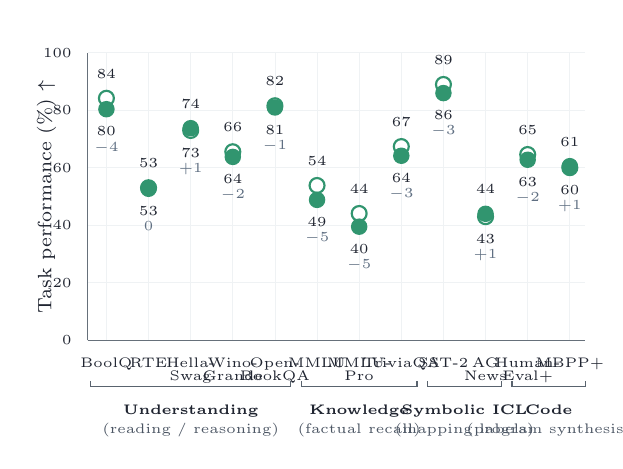
\begin{tikzpicture}[x=1cm,y=1cm]
  % 0.516 x 5.5 in = 7.21 cm: authored at final manuscript width.
  \path[use as bounding box] (0,0) rectangle (7.20,5.25);

  \def\axisx{0.76}
  \def\axisr{7.08}
  \def\ybot{1.28}
  \def\ytop{4.93}
  \def\xstart{1.00}
  \def\xstep{0.535}

  \foreach \i in {0,...,11}{
    \pgfmathsetmacro{\xx}{\xstart + \xstep*\i}
    \draw[grid line] (\xx,\ybot) -- (\xx,\ytop);
  }
  \foreach \v in {0,20,40,60,80,100}{
    \pgfmathsetmacro{\yy}{\ybot + (\ytop-\ybot)*\v/100}
    \draw[grid line] (\axisx,\yy) -- (\axisr,\yy);
    \node[anchor=east,text=FigureInk,font=\AxisTick] at ({\axisx-0.08},\yy) {\v};
  }
  \draw[axis line] (\axisx,\ybot) -- (\axisx,\ytop);
  \draw[axis line] (\axisx,\ybot) -- (\axisr,\ybot);
  \node[rotate=90,anchor=center,text=FigureInk,font=\fontsize{7.0}{7.6}\selectfont]
    at (0.24,{(\ybot+\ytop)/2}) {Task performance (\%) $\uparrow$};

  \newcommand{\dotpair}[6]{%
    \pgfmathsetmacro{\xx}{\xstart + \xstep*#1}%
    \pgfmathsetmacro{\yo}{\ybot + (\ytop-\ybot)*#2/100}%
    \pgfmathsetmacro{\yp}{\ybot + (\ytop-\ybot)*#3/100}%
    \pgfmathsetmacro{\yhi}{max(\yo,\yp)}%
    \pgfmathsetmacro{\ylo}{min(\yo,\yp)}%
    \draw[connector] (\xx,\yo) -- (\xx,\yp);%
    \draw[draw=FigureGreen,fill=white,line width=0.78pt]
      (\xx,\yo) circle[radius=2.70pt];%
    \filldraw[draw=FigureGreen,fill=FigureGreen,line width=0.55pt]
      (\xx,\yp) circle[radius=2.70pt];%
    \node[anchor=south,text=FigureInk,font=\ValueLabel]
      at (\xx,{\yhi+0.13}) {#4};%
    \node[anchor=north,text=FigureInk,font=\ValueLabel]
      at (\xx,{\ylo-0.10}) {#5};%
    \node[anchor=north,text=FigureDelta,font=\DeltaLabel]
      at (\xx,{\ylo-0.29}) {#6};%
  }

  \dotpair{0}{84.2}{80.4}{84}{80}{$-$4}
  \dotpair{1}{53.06859206}{52.70758123}{53}{53}{0}
  \dotpair{2}{73.0}{73.8}{74}{73}{+1}
  \dotpair{3}{65.6}{63.8}{66}{64}{$-$2}
  \dotpair{4}{81.6}{81.0}{82}{81}{$-$1}
  \dotpair{5}{53.85791923}{48.84784402}{54}{49}{$-$5}
  \dotpair{6}{44.11120101}{39.52275182}{44}{40}{$-$5}
  \dotpair{7}{67.4}{64.2}{67}{64}{$-$3}
  \dotpair{8}{89.0}{86.0}{89}{86}{$-$3}
  \dotpair{9}{43.0}{44.0}{44}{43}{+1}
  \dotpair{10}{64.63414634}{62.80487805}{65}{63}{$-$2}
  \dotpair{11}{60.05291005}{60.58201058}{61}{60}{+1}

  \newcommand{\bench}[2]{%
    \pgfmathsetmacro{\xx}{\xstart + \xstep*#1}%
    \node[anchor=north,align=center,text=FigureInk,font=\DatasetLabel]
      at (\xx,1.18) {#2};%
  }
  \bench{0}{BoolQ}
  \bench{1}{RTE}
  \bench{2}{Hella-\\Swag}
  \bench{3}{Wino-\\Grande}
  \bench{4}{Open-\\BookQA}
  \bench{5}{MMLU}
  \bench{6}{MMLU-\\Pro}
  \bench{7}{TriviaQA}
  \bench{8}{SST-2}
  \bench{9}{AG\\News}
  \bench{10}{Human-\\Eval+}
  \bench{11}{MBPP+}

  \newcommand{\family}[4]{%
    % Keep a visible gap between adjacent family brackets.  The previous
    % 0.30-cm extension made neighboring brackets overlap, obscuring the four
    % capability groups even though the labels themselves were present.
    \pgfmathsetmacro{\xl}{\xstart + \xstep*#1 - 0.20}%
    \pgfmathsetmacro{\xr}{\xstart + \xstep*#2 + 0.20}%
    \pgfmathsetmacro{\xc}{(\xl+\xr)/2}%
    \draw[family bracket]
      (\xl,0.76) -- (\xl,0.69) -- (\xr,0.69) -- (\xr,0.76);%
    \node[anchor=north,text=FigureInk,font=\FamilyLabel]
      at (\xc,0.58) {#3};%
    \node[anchor=north,align=center,text=FigureSecondary,font=\FamilyDescription]
      at (\xc,0.35) {#4};%
  }
  \family{0}{4}{Understanding}{(reading / reasoning)}
  \family{5}{7}{Knowledge}{(factual recall)}
  \family{8}{9}{Symbolic ICL}{(mapping labels)}
  \family{10}{11}{Code}{(program synthesis)}
\end{tikzpicture}
\end{document}
